\chapter{Metodologia e Ferramentas}


\section{Sinais de Tempo Discreto e Transformada Discreta de \textit{Fourier}}

	\subsection{Problema da Amostragem de Sinal Contínuo}
	\label{secao-sinal-continuo}
	
		Antes da abordagem do efeito seletivo em frequência em estudo, devemos abordar de forma sucinta um importante teorema que serve de ponte entre os mundos do tempo contínuo e de tempo discreto\footnote{Um sinal contínuo amostrado é uma sequência de impulsos, enquanto que um sinal em tempo discreto apresenta a mesma informação em uma sequência de números. Todos os conceitos aplicados a sinais amostrados se aplicam a sinais em tempo discreto.\cite{haykin2001sinais}}: O teorema da Amostragem. 
		
		Sabe-se que a transformada de Fourier de um sinal de tempo contínuo $x(t)$ é dada por:
		
		\begin{equation}
			X(f) = \mathscr{F} [x(t)] = \int_{-\infty}^{\infty}x(t)e^{-j2\pi f t}dt
			\label{eq:1}
		\end{equation}
		
		Na maioria das vezes, um sinal de áudio dificilmente terá uma representação analítica, como geralmente ocorre com os sinais no mundo real. Assim, teremos que representar o sinal $X(f)$ numa quantidade finita de frequências, em outras palavras, é possível determinar somente um número finito de amostras de $X(f)$.
		
		Nesse caso, uma forma de amostrar um sinal é através do concatenamento do sinal original $x(t)$ por um trem de impulsos periódicos $\delta_{T_s}(t)$. O período, $T_s$, é chamado de intervalo de amostragem: é o espaçamento entre amostras consecutivas tomadas de $x(t)$.
		
		O sinal amostrado $x_s(t)$ é dado matematicamente pela seguinte equação, para $n\in \Z$:
		
		\begin{equation}
			x_s(t) = \sum_{n=-\infty}^{\infty}x(nT_s)\delta(t-nT_s)
			\label{eq:2}
		\end{equation}
		
		A transformada de Fourier neste caso para o sinal $x_s(t)$, pode ser obtida da seguinte forma:
		
		\begin{equation}
			\begin{aligned}
				&X_s(f) = \mathscr{F}[x(t)\delta_{T_s}(t)] = X(f)\ast\Delta_{T_s}(f)= 
				\\
				&X(f)\ast f_s\sum_{k=-\infty}^{\infty}\delta(f-kf_s) = \boxed{f_s\sum_{k=-\infty}^{\infty}X(f-kf_s)}
				\label{eq:3}
			\end{aligned}
		\end{equation}
		
		Nota-se que o sinal $X_s(f)$ é periódico com período $f_s$ hertz. Considerando uma largura espectral do sinal $X(f)$ como B, em que $X(f) = 0$ para $|f|\ge f_s/2$ - isto é, $B \le f_s/2$, ou, de forma análoga $f_s \ge 2B$.
		
		Dessa forma podemos avaliar o sinal $X(f)$ como sendo:
		
		\begin{equation}
			X(f) = T_s.X_s(f)
			\label{eq:4}
		\end{equation}, para $|f|<f_s/2$, se $f_s \ge 2B$
		
		Ou seja, se $f_s\ge 2B$, é possível obter X(f) a partir do sinal discreto $X_s(f)$ que, por consequência, reconstruir $x(t)$ a partir de $x_s(t)$. Esse resultado é conhecido como \textbf{teorema da amostragem}.
		
		No nosso caso concreto, teremos que utilizar esses conceitos para avaliar uma taxa de amostragem coerente bem como conceitos relativos ao tipo de método usado para representar digitalmente amostras de um sinal analógico, por exemplo o som da guitarra ou de uma amostra musical.
		
		Vale também salientar que o espectro $X_s(f)$ pode ser obtido calculando-se diretamente a transformada de Fourier de $x_s(t)$ usando-se as equações \eqref{eq:1} e \eqref{eq:2}, pode-se mostrar que:
		
		\begin{equation}
			X_s(f) = \int_{-\infty}^{\infty}\underbrace{x_s(t)}_{x(nT_s)\delta(t-nT_s)}e^{-j2\pi ft}dt = \sum_{n=-\infty}^{\infty}x(nT_s)e^{-j2\pi fnT_s}
			\label{eq:5}
		\end{equation}
		
		Substituindo na equação \eqref{eq:4}, para $|f|<f_s/2$, se $f_s\ge 2B$ temos:
		
		\begin{equation}
			X(f) = T_s\sum_{n=-\infty}^{\infty}x(nT_s)e^{-j2\pi fnT_s}
			\label{eq:6}
		\end{equation}
		
		
		Nota-se que a equação \eqref{eq:6} pode ser usada também para o cálculo numérico de $X(f)$\footnote{A expressão dada equação \eqref{eq:6} para $X(f)$ é a mesma que se obtém utilizando a regra do trapézio para solucionar numericamente a equação \eqref{eq:1}, contudo com essa abordagem é mais difícil visualizar com clareza aspectos importantes e limitações desse cálculo numérico}.
		
		
	\subsection{Efeito do Janelamento}
	\label{secao-janelamento}
		
		Apesar dessa discretização do sinal ainda tratamos de um sinal com somatório infinito, que, em geral, não será possível de ser calculado. Portanto, esse somatório precisa ser truncado, e consequentemente, não se terá mais a igualdade da equação \eqref{eq:6}, mesmo que $X(f) = 0$ para $|f| \ge f_s/2$.
		
		Uma consideração acerca desse truncamento é dada pela equação abaixo, para $n\in [0,N-1]$:
		
		\begin{equation}
			\label{eq:7}
			\hat{X}(f) = T_s\sum_{n=0}^{N-1}x(nT_s)e^{-j2\pi fnT_s}
		\end{equation}
		
		
		Uma forma de tratar o truncamento, por questões de continuidade manter a continuidade do sinal amostrado, é considerá-lo como resultante do truncamento do sinal $x(t)$, realizado por meio da multiplicação desse sinal com um sinal $w(t)$ de duração finita, geralmente $w(t)$ é um sinal retangular. Chamaos o sinal $w(t)$ de sinal-janela ou, simplesmente janela.
		
		Assim definimos o sinal $x_w(t)$ como sendo:
		
		\begin{equation}
			\label{eq:8}
			x_w(t) = w(t)x(t)
		\end{equation}
		
		Escolhendo um tempo de janelamento $Tw = NT_s$, tem-se que $x_w(nT_s) = 0$ para $n \notin [0,N-1]$. Assim, substituindo na equação \eqref{eq:6} podemos obter uma aproximação $\hat{X}(f)$, para $|f|<f_s/2$, dada por:
		
		\begin{equation}
			\label{eq:9}
			\hat{X}(f) = T_s \sum_{n=0}^{N-1}x_w(nT_s)e^{-j2\pi fnT_s}
		\end{equation}
		
		Podemos considerar que a aproximação da equação \eqref{eq:9} é idêntica a fornecida pela equação \eqref{eq:7} pois, considerando que o sinal $w(t)$ é uma janela retangular\footnote{$w(t) = rect\left(\frac{t-T_w/2}{T_w}\right) = \begin{cases}1,\, 0\le t < T_w \\ 0, \,\, c.c\end{cases}$}, então $x_w(nT_s) = x(nT_s)$, para $n\in [0,N-1]$.
		
		Todavia o somatório dessas equações, embora finito, não poderá ser transofrmado em uma expressão analítica válida para qualquer $|f|<f_s/2$. Isto é, para cada valor de $f$ dado, para o qual se deseje determinar $\hat{X}(f)$, será preciso calcular o referido somatório, o que não é nada prático.
		
		Uma alternativa é o cálculo de $\hat{X}(f)$ para valores de $f$ espaçados de:
		
		\begin{equation}
			\label{eq:10}
			\Delta f = \frac{f_s}{N}
		\end{equation}
		
		Ou seja, para $f = k\Delta f$, $k\in \Z$
		
		Assim, usando a equação\footnote{Sendo $|f|<f_s/2$ e $f = k\Delta f$, portanto $|f| = |k||f_s/2|\Rightarrow |k|>N/2$.} \eqref{eq:9}, para $|k|\le N/2$:
		
		\begin{equation}
		\label{eq:11}
		\hat{X}(k\Delta f) = T_s \sum_{n=0}^{N-1}x_w(nT_s)e^{-j2\pi k \frac{f_s}{N}nT_s} = T_s\sum_{n=0}^{N-1}x_w(nT_s)e^{-j\frac{2\pi}{N}kn}
		\end{equation}
		
		
		Finalmente definindo o sinal de tempo discreto $x_w[n] = x_w(nT_s)$, a equação \eqref{eq:11} pode ser reescrita como:
		
		\begin{equation}
		\label{eq:12}
		\hat{X}(k\Delta f) = T_s\sum_{n=0}^{N-1}x_w[n]e^{-j2\pi k \frac{f_s}{N}n}
		\end{equation}
		
		O somatório dessa equação é a transformada de Fourier discreta (DFT - \textit{discrete Fourier transform}).
		
		O conhecimento desse conceito matemático, bem como suas limitações quanto aos problemas de janelamento e de sobreposição espectral (aliasing) são fundamentais para entendimento das próximas atividades efetuadas.
	
\section{Filtros Digitais}

	\subsection{Conceitos Iniciais}
	
		Os filtros digitais não contém uma implementação física em si, diferentemente dos filtros analógicos constituídos, geralmente, de associação de resistores e capacitores. Eles são construídos através de algoritmos.
		
		Para que isso possa ocorrer é necessário que o sinal de áudio (analógico) seja devidamente convertido em um sinal digital. esse sinal portanto convolui por um algoritmo de filtro adequado.
		
		De maneira geral, o projeto de um filtro consiste em obter os coeficientes para os filtros. Isso é realizado através de uma equação chamada de equação das diferenças. O processo pode ser simplesmente realizado pela equação (\ref{eq-filtro-bas}):
		
		\begin{equation}
			\text{Saida} = \sum_{1}^{n} \text{Coeficiente}_n \text{do filtro} * \text{Amostra}_n
			\label{eq-filtro-bas}
		\end{equation}
		
		Assim, o contexto de um filtro digital estará associado a equações de diferenças (ou funções de transferência no domínio Z) cujo parâmetros (coeficientes) serão calculados com o objetivo de discriminar (extrair, atenuar, etc.) determinadas componentes espectrais presentes em um sinal ou uma informação no mesmo sentido dos filtros analógicos, sem a necessidade de um circuito (\textit{hardware}) adicional. Em outras palavras, o filtro digital será uma rotina adicional agregada ao algoritmo responsável pela realização do sistema proposto em questão.
		
	\subsection{Filtros IIR}
	\label{secao-IIR-section}
		
		Os filtros digitais de resposta infinita ao impulso (\textit{Infinite Impulse Response - IIR}), também conhecidos como filtros recursivos ou autorregressivos, são modelados pela equação de diferença (\ref{eq1-iir}) ou pela função de transferência (\ref{eq2-iir-tf}), em que basicamente os valores dos coeficientes dos modelos define a natureza do filtro (passa-baixa; passa-alta; passa-faixa; rejeita-faixa).
		
		A denominação de IIR se deve que a saída do modelo decai para um valor nulo em um tempo infinito em resposta a um impulso aplicado na entrada filtro correspondente.
		
		\begin{equation}
			y(k) = \frac{1}{a_0}\left(\sum_{m=0}^{M}b_mx(k-m)-\sum_{n=1}^{N} a_ny(k-n)\right)
			\label{eq1-iir}
		\end{equation}
		
		\begin{equation}
			D(z) = \frac{y(z)}{x(z)} = \frac{b_0 + b_1z^{-1}+...+ b_mz^{-m}}{a_1z^{-1}+ a_nz^{-n}}
			\label{eq2-iir-tf}
		\end{equation}
		
		Resumidamente, a forma usual de calcular os coeficientes de um filtro digital IIR consiste em utilizar o modelo de um filtro analógico, e aplicar uma transformada Z via aproximação retangular ou trapezoidal \cite{Oppenhein1998}.
		
		Notoriamente, uma das vantagens na utilização dos filtros IIR é que eles resultam em comprimentos (quantidade de coeficientes) de filtro menor do que o filtro FIR correspondente, porém, esta melhoria é obtida às custas de distorção de fase e um transitório que não se limita a um intervalo de tempo finito \cite{Roberts1987}.
		
		Adicionalmente, conforme veremos na seção (\ref{comb-filter}) deste capítulo, um exemplo clássico de um filtro IIR é o Filtro Pente, pois se estável, a resposta simplesmente consiste em repetir 'series de impulsos que decrescem em amplitude com o tempo.
		
		
	\subsection{Filtros FIR}
		
		\begin{figure}[!htb]
			\centering
			\subfigure[\textbf{fluxo de sinais}]{
			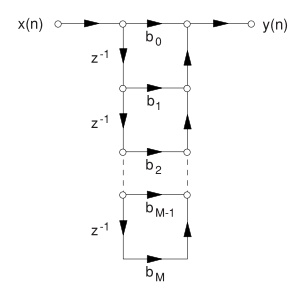
\includegraphics[scale=0.5]{./figuras/FIR-diagrama-fluxo-sinais.png}
			\label{figura1-fir}}
			\qquad
			\subfigure[\textbf{diagrama de blocos}]{
			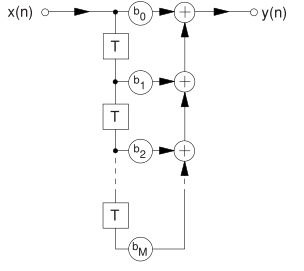
\includegraphics[scale=0.5]{./figuras/FIR-diagrama-blocos.png}
			\label{figura2-fir}}
			\caption{Diagrama de fluxo de sinais e diagrama de blocos de um filtro FIR}
			\label{fig01}	
		\end{figure}
		
		O lóbulo principal da janela retangular tem aproximadamente a metade da largura do lóbulo principal da janela \textit{Hamming};
		
		Os lóbulos laterais da janela \textit{Hamming}, em relação ao lóbulo principal, são muitos reduzidos em comparação com os da janela retangular. Especificamente, o pico de amplitude do primeiro lóbulo lateral da janela retangular está somente aproximadamente 13 dB abaixo do pico do lóbulo principal, ao passo que o valor correspondente para a janela \textit{Hamming} é de aproximadamente 40 dB.
		
		É devido a esta último ponto que a janela \textit{Hamming} reduz as oscilações na resposta em frequência de um filtro digital FIR. Todavia, há um preço a ser pago por esta melhoria, a saber, uma faixa de transição mais larga no espectro do filtro.\cite{haykin2001sinais}
	
		Vantagens:
		\begin{itemize}
			\item Um filtro não recursivo como o filtro FIR é inerentemente estável. Conforme pode ser visto na função de transferência ela é especificada em termos do zeros apenas no plano-z. Logo não há grandes preocupações em termos da escolha dos coeficientes que possam causar instabilidade no sistema, posto que seu LGR encontra-se estritamente dentro do semi-plano esquerdo do domínio-z.
			\item O filtro FIR (resposta ao impulso) tem forma simétrica no seu espectro de frequência. Isso produz uma característica de fase linear ideal, ou seja, é equivalente a puramente um atraso temporal em todas as componentes de frequência passando pelo filtro. Em outras palavras, podemos dizer que o filtro FIR não tem \textit{distorção de fase} \cite{Lynn1998}.
		\end{itemize}
	
	\subsection{Filtros Adaptativos}
	
		Os filtros adaptativos são constituídos, geralmente, por estruturas FIR, em que os coeficientes dos modelos associados são modificados conforme um procedimento adaptativo. essa modalidade de filtro geralmente é empregada nos seguintes contextos (\textit{lista não exaustiva}):
		
		\begin{itemize}
			\item Como procedimento alternativo na obtenção de valores dos coeficientes de um determinado filtro FIR, em que padrões de entrada e saída conhecidos são utilizados para estabelecer os valores dos coeficientes do filtro em questão;
			\item Cancelamento ou redução de ecos/barulhos de um determinado ambiente;
			\item Na modelagem de sistemas dinâmicos; e
			\item Como modelagem básica de representações de redes neurais artificiais.
		\end{itemize}
	
		A equação () representa o modelo de um filtro FIR, em que $W_m(k)$ denota os valores dos coeficientes do filtro em um instante de tempo $k$. 
		
		\begin{equation}
			\label{eq1-filtroadap}
			y(k) = \sum_{m=0}^{M} W_m(k)x(k-m)
		\end{equation}
		
		A diferença ou erro $\epsilon(k)$ entre o valor de padrão desejado d(k) para a a resposta do filtro e a informação da saída atual $y(k)$ do modelo associado é expressa por:
		
		\begin{equation}
			\label{eq2-filtroadap}
			\epsilon(k) = d(k)- y(k)
		\end{equation}
		
		Basicamente para ajustar os valores dos coeficientes de um filtro adaptativo tipicamente utiliza o método do gradiente para essa finalidade (fonte....), sendo o critério da somatória do erro quadrático de $\epsilon_(k)$ frequentemente utilizado na etapa de adaptação.
		
		Vale salientar, que alguns sistemas de comunicação de voz utilizam filtros adaptativos com o objetivo de cancelar ou reduzir ecos ou barulhos do ambiente. Nesse contexto, foi pensado inicialmente a utilização desse modelo de filtro para o projeto. No entanto, será explicado mais a frente a não adoção desse modelo, bem como pela utilização de um filtro FIR típico.
		
	\subsection{Filtro Pente - \textit{Comb Filter}}
	\label{secao-comb-filter}
		
		Em termos práticos \textit{comb filter} ou “filtro pente” é uma versão atrasada do mesmo sinal, causando uma  interferência construtiva ou destrutiva de dois sons tocados simultaneamente, porém com atraso entre um para o outro. 
		
		Nesse sentido, há basicamente dois tipos de \textit{comb filters}: o (\textit{feedback comb filter}) e (\textit{feedforward comb filter}). Resumidamente, os nomes referem-se à direção em que os sinais são atrasados antes de serem adicionados à entrada. O primeiro tipo considera em adicionar a saída do filtro a entrada imediatamente posterior, enquanto o segundo considera apenas adicionar à saída do filtro as entradas presente e a mesma entrada atrasada.
		
		\begin{figure}[hbt]
			\centering
			\subfigure[\textbf{Feedback comb-filter}]{
				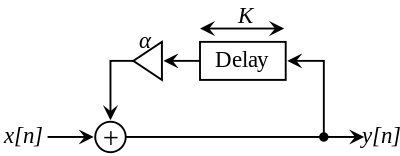
\includegraphics[scale=0.5]{./figuras/Comb_filter_feedback.png}
				\label{fig01a-combfilter}
				}
			\qquad
			\subfigure[\textbf{Feedforward comb-filter}]{
				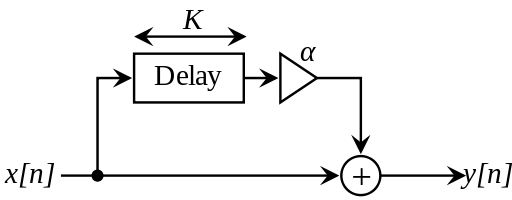
\includegraphics[scale=0.5]{./figuras/Comb_filter_feedforward.png}
				\label{fig01b-combfilter}
			}
			\caption{Filtro Pente - \textit{Comb Filter} - Formas de Realimentação}
			\label{fig01-combfilter}
		\end{figure}
		
		Como já informado, o caso do filtro pente com realimentação na saída, é um caso especial de um Filtro de Resposta Infinita (\ref{IIR-section}), posto que pode ser observado uma figura de atraso (\textit{delay}) no sentido de realimentação no sistema. Este filtro pode ser um modelo físico computacional de "séries de ecos", os quais decaem exponencialmente, bem como espaçados uniformemente no tempo \cite{JuliusO.Smith2010}.
		
		
		Continuando a análise do modelo do referido filtro, ve-se que a estrutura geral de um sistema de realimentação de um \textit{ feedback comb filter} pode ser mostrado através da figura \ref{fig01a-combfilter}. Além disso pode ser descrito pela seguinte equação\footnote{Para um critério de estabilidade o coeficiente $\alpha$ da equação \ref{eq01-combfilter} tem que ser menor ou igual a 1 (0db).} de diferenças \ref{eq01-combfilter}:
				
		\begin{equation}
			\label{eq01-combfilter}
			y[n] = x[n] + \alpha y[n-K]
		\end{equation}
		
		Se rearranjarmos os termos da equação para que todos as variáveis em $y$ fiquem do mesmo lado da equação e, na sequência, aplicamos a transformada Z em ambos os membros, teremos:
		
		\begin{equation}
			\label{eq02-combfilter}
			(1-\alpha z^{-K})Y(z) = X(z)
		\end{equation}
		
		Finalmente temos a função de transferência (\ref{eq03-combfilter}) correspondente ao sistema:
		
		\begin{equation}
			\label{eq03-combfilter}
			H(z) = \frac{Y(z)}{X(z)} = \frac{1}{1-\alpha z^{-K}} = \frac{z^K}{z^K-\alpha}
		\end{equation}
		
		Uma das formas de estimar a resposta de magnitude em função do valor do tempo de delay $K$ e fator de atenuação/ganho $\alpha$ é expressar $ H(z) $ em termos de módulo $|H(K,\alpha)|$, bem como, de maneira conveniente, utilizando uma substituição $ z = e^{j\omega} $.
		
		\begin{equation}
			|H(e^{j\omega})| = \frac{1}{|1-\alpha e^{-j\omega K}|},
			\qquad
			-\pi\leq \omega \leq \pi
			\label{eq04-combfilter}
		\end{equation}
		
		Nota-se pela expressão do ganho dada pela equação (\ref{eq04-combfilter}) que seu valor tem valores de resposta \textbf{periódica} indo de um valor mínimo e subindo para um valor máximo.
		
		Supondo o valor de $\alpha = 1$ ($0$ dB), para simplificar os cálculos, a amplitude da resposta reduz-se a:
		
		\begin{equation}
			\label{eq05-combfilter}
			H(w) = \frac{1}{2|sin(\omega M/2)|}
		\end{equation}

		Note ainda que para $\alpha > 0$ são produzidos picos de ressonância em:
		
		\begin{equation}
			\begin{aligned}
				\sin(\omega K/2) &= 0 \\
				\omega \frac{K}{2} &= p\pi,\quad p=0,1,2,...,K-1\\
				w_p &= 2\pi\frac{p}{K}
			\end{aligned}
		\end{equation}
		
		Ou seja, em todos harmônicos pares do filtro.
				
		Ademais, esses filtros são utilizados em toda sorte de efeitos de sons, principalmente no universos de instrumentos musicais. Vários desses filtros podem ser usados por exemplo para simular uma reverberação.
		
		Por último, vamos falar do modelo proposto para o projeto deste trabalho, no qual consiste de uma versão mais generalista do \textit{feedback comb-filter}. Este modelo propõe a alocação de um filtro casual $H_l(z)$ na malha de realimentação, em vez de apenas um ganho de atenuação $\alpha$. A função de transferência \ref{eq02-combfilter} pode ser então reescrita como:
		
		\begin{equation}
			H(z) = \frac{1}{1-H_l(z)z^{-K}}
		\end{equation}
		
		\begin{mymdframed}{NOTA}
			Para o critério de estabilidade do sistema, a amplitude de resposta do filtro $ H_l(z) $ deverá ser menor que 1 em todas as frequências, i.e, $ |H_l(e^{j\omega T})| < 1, \forall \omega T \in [-\pi,\pi)$
		\end{mymdframed}
		
		
\section{Conversão Analógica Digital}
	
	\subsection{Considerações Iniciais}
		
	\subsection{Conversão Por Aproximações Sucessivas}
		
		Resumidamente, conforme pode ser observado na figura \ref{conv-aprox-sucessivas1} este tipo de conversor utiliza uma técnica de realimentação para relacionar uma voltagem analógica de entrada com um código digital correspondente (conforme os N bits de resolução do conversor). No início do processo de conversão o \textit{shift register} e o \textit{holding register} são zerados. Na primeira etapa de conversão o MSB (bit mais significativo) do \textit{holding register} é colocado em	nível alto (1 lógico) e os demais mantidos em nível baixo (0 lógico). É, então, realizada uma comparação entre o resultado de saída do conversor D/A ($V_O$) e o sinal de entrada ($V_{IN}$). Se $V_O < V_IN$, o nível “1” é mantido para o MSB, caso contrário é substituído por “0”. A etapa seguinte repete o mesmo processo para o 2-SB. Isso continua até que todos os $N$ bits tenham sido verificados. A decisão de manter o nível lógico “1” ou substituir por “0” é realizada pelo comparador e pelo registrador de aproximação sucessiva. O controle lógico controla o início e o fim de cada etapa de aproximação e o resultado destas etapas são retidas no \textit{holding register}. O sinal de saída é válido apenas quando todo o processo for concluído e isto é sinalizado pelo sinal de \textit{status} do controle lógico.
		
		\begin{figure}[!ht]
			\centering
				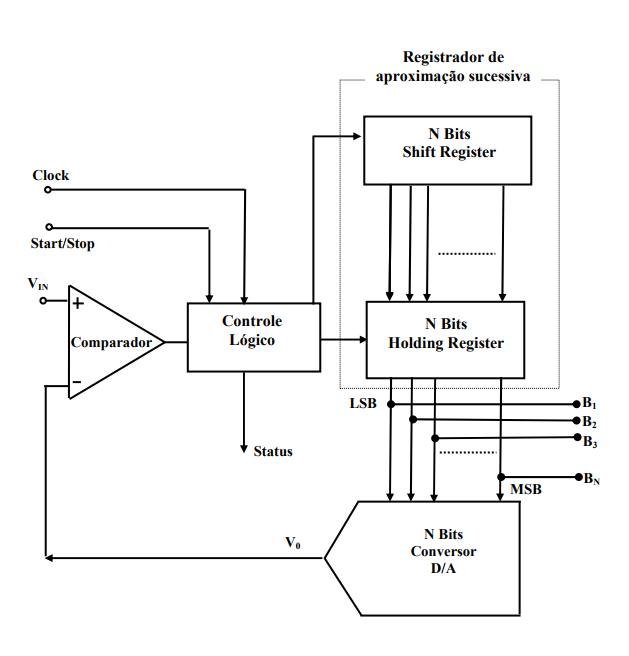
\includegraphics[scale=0.5]{./figuras/aprox-sucessivas-conv-ad.png}
				\caption{Conversor A/D de aproximações sucessivas.}
				\label{conv-aprox-sucessivas1}
		\end{figure}
	
	\subsection{Dificuldades Práticas de Conversores ADs}
		
		Apesar do princípio de funcionamento de um conversor AD ser relativamente simples, em suma, a operação desse dispositivo não é uma simples conexão de um sinal analógico na entrada de um microcontrolador. Listamos aqui algumas das dificuldades naturalmente encontradas:
		
		\begin{itemize}
			\item \textbf{Intervalo de Tensão de Entrada}: Bem, se conectarmos uma guitarra que produz em seus captadores digamos valores em $\pm 100 mV$ nãó será possível conectar diretamente essa tensão num conversor de um microcontrolador que espera valores entre $1V$ a $3V$. Neste caso é necessário que o sinal da guitarra seja amplificado e modificado para que ele "ajuste-se" ao ADC.
			
			\item \textbf{Tensão de Referência}: Um ADC não tem uma noção absoluta de tensão, em outras palavras, sua tarefa é comparar sua entrada com a tensão de referência e sua saída numa proporção de 2. Assim, uma saída precisa recai na qualidade da referência e isso limita a acurácia\footnote{text} em geral.
			
			\item  \textbf{Ruído e filtragem}: Sinais no mundo real contém frequências indesejadas, no nosso caso, uma guitarra ligada numa cadeira de pedais com fontes de alimentação cuja frequência da rede elétrica gira torno de $50-60Hz$. Nesse caso filtros são necessários para remover esse ruído ainda de iniciar a conversão ADC propriamente dita. Vale apontar, conforme seção \ref{secao-janelamento} que um filtro passa-baixa é também necessário para evitar-se o efeito de \textit{aliasing}.
		\end{itemize}
			
			

\section{Conversão Digital Analógica}

\section{Comunicação Serial I2C}
	
\section{Ferramentas Computacionais}

	\subsection{\textit{Code Compose Studio}}
	
	\subsection{\textit{WinFilter}}
